\graphicspath{{./design/}}

\chapter{Design}
% {{{
\label{cha:design}

% {{{

The goal of the visualisation aspect of the system is to provide a way to
easily interpret the molecular data. The visualisation techniques chosen either
support the compression aspect of the water compression system, or allow for
general interpretation of data. The main challenge to effective visualisation
of the data is the density of atoms potentially resulting in a cluttered view.

A brief overview of the entire system is provided in Section
\ref{sec:design_overview}, while Section \ref{sec:design_visualisation}
provides more detail on the visualisation components of the system. Section
\ref{sec:design_summary} briefly summarises this chapter.

% }}}

\section{System overview}
% {{{
\label{sec:design_overview}

% {{{

The design of the system has been broken down into a number of components:

\begin{itemize}

  \item \textbf{Quantiser} - quantises and dequantises the points for each
  frame.

  \item \textbf{I/O} - handles the input and output of molecular data files,
  i.e. the PDB and DCD files.

  \item \textbf{Water cluster extractor} - groups water molecules together to
  form water clusters, these water clusters are predominantly used for
  intraframe prediction.

  \item \textbf{Verifiers} - verify and record various aspects of the
  compression system such as compression results and quantisation error.

  \item \textbf{Arithmetic coders} - encodes and decodes symbols to and from
  compressed bit streams.

  \item \textbf{Visualisation} - renders and allows the user to explore the
  simulation data.

  \item \textbf{Compressors} - item drivers behind the compression system,
  calls and executes the functions needed to perform the compression and
  decompression.

\end{itemize}

Figure \ref{fig:design_overview} is a schematic diagram of the components in
the system. Julian Kenwood has completed the green areas, Keegan Smith has
completed the cyan areas, while Min-Young Wu has completed the red areas. The
Quantiser, I/O and Water cluster extractor components are used by both the
compressors and the visualisation components. The Verifiers and Arithmetic
coder components are used by the compressors only.

\begin{figure}
  \begin{center}
    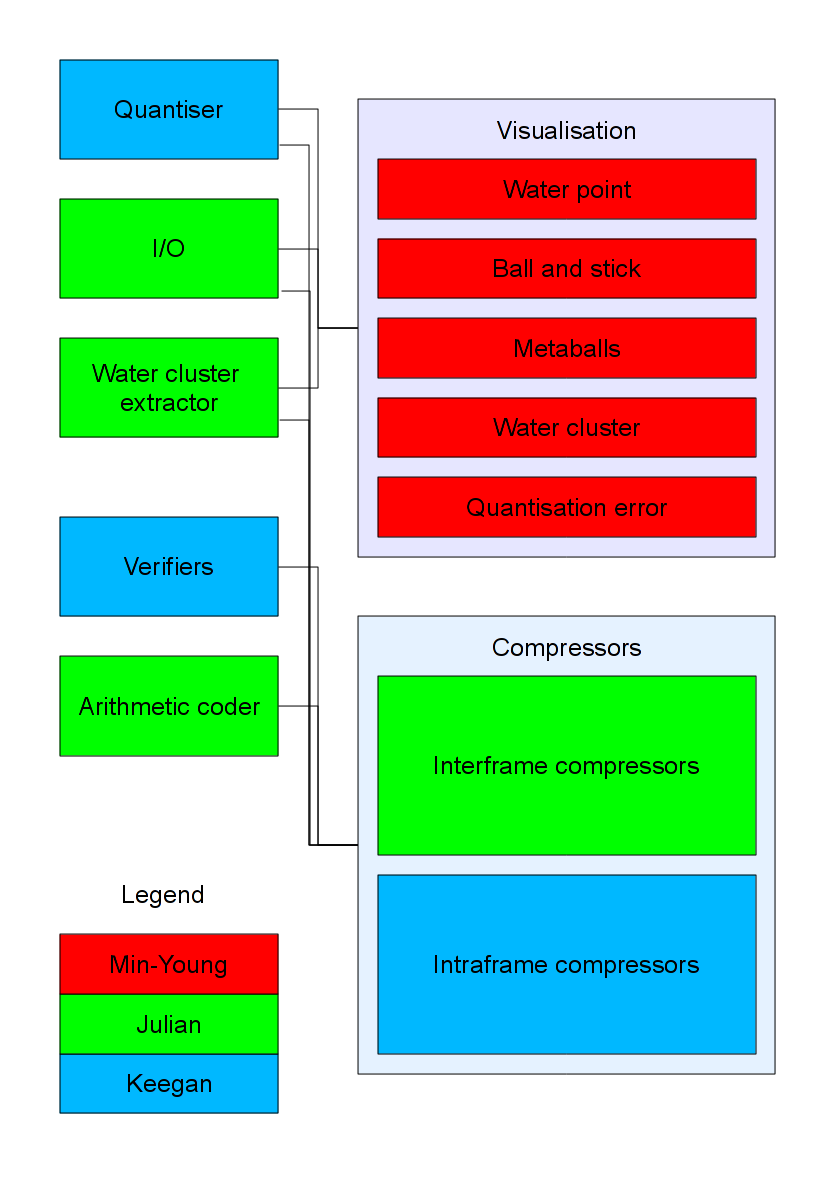
\includegraphics[width=100mm]{breakdown}
  \end{center}
  \caption{Overview of components within the system.}
  \label{fig:design_overview}
\end{figure}

% }}}

% {{{

The visualisation component is divided into a number of sub-components, each of
which represents a different visualisation technique:

\begin{itemize}

  \item \textbf{Water point visualisation} - simple visualisation technique
  using the alpha value effects to convey an idea of the volume.

  \item \textbf{Ball-and-Stick visualisation} - standard approach to
  visualising molecular data.

  \item \textbf{Metaballs visualisation} - determines and renders the surface
  between the water and non-water regions.

  \item \textbf{Water cluster visualisation} - renders the extracted water
  clusters from the frame.

  \item \textbf{Quantisation error visualisation} - shows the error resulting
  from quantising and dequantising the molecular data.

\end{itemize}

All the visualisation sub-components uses the Quantiser and I/O components, but
only the Water cluster visualisation uses the Water cluster extractor
component.

% }}}

% }}}

\section{Visualisation}
% {{{
\label{sec:design_visualisation}

\paragraph{Water point visualisation}
% {{{

This visualisation technique is the simplest visualisation technique in the
system. A single point primitive is rendered for each water molecule, with
non-water molecules being filtered out.

Filtering out the non-water molecules is the first step in reducing visible
clutter. Using a low alpha value per point further reduces clutter by causing
regions where the molecules are not very dense to appear more faintly, the more
densely populated regions are thus emphasised.

While this visualisation technique does allow for the regions of high water
density to be easily identified, the details of the volume are not visible.

% }}}

\paragraph{Ball-and-stick visualisation}
% {{{

The ball-and-stick visualisation is the same as the classical ball-and-stick
representation (Chapter \ref{cha:background}). The atoms are represented by
spheres, the spheres are rendered using different colours and sizes to
represent the different atoms. The bonds between the atoms is represented by a
cylinder.

This visualisation provides more visual information about the water molecules.
Rendering the individual atoms allows for the orientation of the individual
water molecules to be seen.

Showing the individual atoms and orientation exposes the quantisation error
more clearly, thus this visualisation is used in the quantisation experiment
(Chapter \ref{cha:experiment}).

Rendering all the water molecules will cause significant clutter, therefore the
number of molecules to render can be limited from the user interface. This is
simply adjusting the number of molecules rendered.

% }}}

\paragraph{Metaballs visualisation}
% {{{

The metaballs visualisation is an alternative way to visualise the water volume
in the molecular simulation. The aim of the metaballs visualisation is to
separate the regions of water from the regions of non-water. A surface between
the water and non-water regions is extracted and rendered.

The metaballs surface is determined by voxelising the volume, each of the water
molecules then contributes to the voxels around it, indicating that it is
within a region of water. The voxels which are determined to be between a water
and non-water region are then combined to create the final metaballs surface.

The surfaces extracted from volume data are often densely populated with many
triangles. This increases the rendering costs of the surface, thus decreasing
frame rates and interactivity.

The extracted surfaces can be decimated to decrease rendering costs. Decimating
the surface will decrease the number of surface primitives, hence decreasing
the amount of processing required to render the surface, and allowing the
volume to be more easily explored.

An alternative to decimating the surface in order to decrease the surface
complexity, is to decrease the level of sampling. Sampling the volume less
densely results in fewer triangles, but the surface quality will also decrease.

Decimation is preferred over reduced sampling as the surface quality can be
maintained. Reduced sampling would skip over details on the surface, but
decimation would maintain the surface details, thus maintaining surface
quality. The rendering cost is decreased in exchange for computation cost,
where the computation is performed once for every frame, but can be done as a
pre-process.

% }}}

\paragraph{Water cluster visualisation}
% {{{

The water clusters are extracted using the \emph{water cluster extractor}
component of the system. Heuristics are used to connect the water molecules
together to form the water clusters.

The water molecules in a water cluster are joined by cylinders, spheres are
drawn at the end points of the cylinders to represent the water molecules.

Similar to the ball-and-stick visualisation, rendering all the water clusters
will cause significant clutter, therefore the number of clusters to render can
be limited by simply changing a value in the user interface.

This visualisation technique is primarily useful in supporting the compression
components of the system. There has been little research into water clusters in
chemistry, thus it is unlikely that this visualisation technique will be of
interest to chemists.

% }}}

\paragraph{Quantisation error visualisation}
% {{{

Quantisation is the only lossy step in the compression, thus it is important to
show the amount of error that is introduced. The distance between the original
and quantised position of the water molecule is the quantisation error
introduced.

Visualising the error is accomplished by either rendering a point for the water
molecule, or a line between the original and quantised positions. The colour of
the point or line is linked to the magnitude of the error.

Points and lines are rendered instead of spheres and cylinders due to their
smaller visual size. As quantisation is applied to the entire volume, viewing
all the quantisation errors is desired. Using spheres or cylinders would
obscure parts of the volume.

As the errors are uniformly distributed, having the colour linearly
proportional to the error value produces poor results: the large error values
do not stand out clearly. Instead, a stepped colour scale is used so that there
is a larger visual difference between the lower and higher error values.

Figure \ref{fig:design_quantgraph} shows a graph illustrating how the colour is
determined. The colour scale is determined using two error thresholds. If the
error value is less than the lower threshold, then the error is ignored and
nothing is rendered. If the error value is between the two threshold values,
then the colour is determined linearly up till the upper threshold value, where
the colour is set to the final error colour.

\begin{figure}
  \begin{center}
    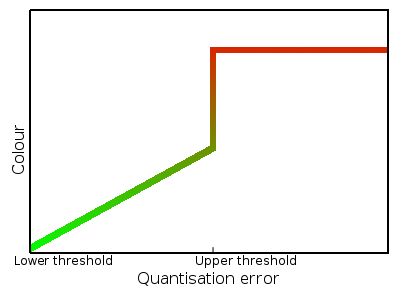
\includegraphics[width=80mm]{quant_colour_graph}
  \end{center}
  \caption{Graph illustrating stepped colour assignment for quantisation error.}
  \label{fig:design_quantgraph}
\end{figure}

This visualisation technique is only useful in supporting the compression
components of the system.

% }}}

% }}}

\section{Summary}
% {{{
\label{sec:design_summary}

Five different visualisation approaches has been identified, all of which
visualises different aspects of the molecular data.

The \emph{water cluster} visualisation provides a quick idea of the volume.

The \emph{ball-and-stick} visualisation provides the most detail by including
all the atoms.

The \emph{metaballs} visualisation simplifies the volume data by identifying
the boundary between water and non-water molecules, and rendering that.

The \emph{water cluster} visualisation renders clusters of water molecules
using cylinders and spheres, the water clusters are used in the intraframe
compression component of the system.

The \emph{quantisation error} visualisation displays the error resulting from
quantisation. Quantisation is the first step in the compression process,
both intraframe and interframe compression.

The \emph{water cluster} and \emph{quantisation error} visualisations are
designed to support the compression components of the system. It is unlikely
that they will be useful outside of the water compression project.

The other three visualisations, \emph{water point}, \emph{ball-and-stick} and
\emph{metaballs} are more generally applicable and thus may be used for viewing
the molecular data.

% }}}

% }}}

